\documentclass{article}
\usepackage{graphicx}
\usepackage{latexsym}
\author{Chang Liu}
\title{Reading Note for CLRS\footnote{Introduction to algorithm}{ }  Chapter 32}
\begin{document}
\maketitle

1) pattern P \textbf{occurs with shifts s} in text T(or, pattern P \textbf{occurs beginning at position s+1} in text T) if $0\le{s}\le{n-m}$ and $T[s+1..s+m] = P[1..m]$

2) w is a \textbf{prefix} of a string $x$, denoted $w \sqsubset x$ %\sqsubset, \sqsupset%


\begin{center}
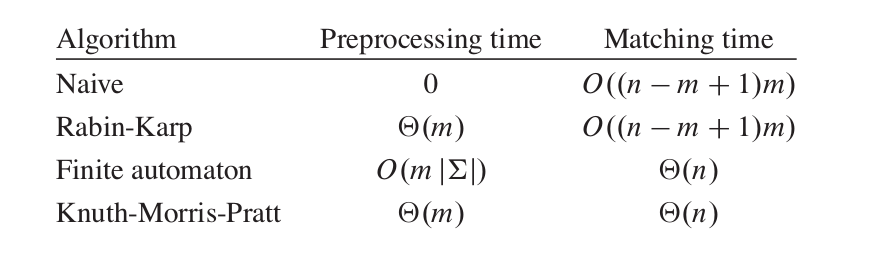
\includegraphics[scale=0.3]{ch32_p1.png}
\end{center}


\end{document}